\documentclass{article}
\usepackage[utf8]{inputenc}
\usepackage{listings}
\usepackage{CJKutf8}
\usepackage{amsmath}
\usepackage{graphicx}
\usepackage[export]{adjustbox}
\title{Lab2 Report}
\author{b09901142 EE3 呂睿超}
\date{October 2022}

\usepackage{xcolor}

\definecolor{codegreen}{rgb}{0,0.6,0}
\definecolor{codegray}{rgb}{0.5,0.5,0.5}
\definecolor{codepurple}{rgb}{0.58,0,0.82}
\definecolor{backcolour}{rgb}{0.8,0.9,0.8}

\lstdefinestyle{mystyle}{
    backgroundcolor=\color{backcolour},   
    commentstyle=\color{codegreen},
    keywordstyle=\color{magenta},
    numberstyle=\tiny\color{codegray},
    stringstyle=\color{codepurple},
    basicstyle=\ttfamily\footnotesize,
    breakatwhitespace=false,         
    breaklines=true,                 
    captionpos=b,                    
    keepspaces=true,                 
    numbers=left,                    
    numbersep=5pt,                  
    showspaces=false,                
    showstringspaces=false,
    showtabs=false,                  
    tabsize=2
}

\lstset{style=mystyle}





\begin{document}
\begin{CJK*}{UTF8}{bsmi}
\maketitle

\section{Superdense Coding}
\subsection{(a)}
\begin{enumerate}
\item In order to implement a 4-bit classical string teleport, I used the superdense coding architecture taught in class twice as two channels. Each of it teleport a segment of 2-bit string. 
\item The Python implementation of superdense coding is in \emph {Appendix 1}:

\item Then I use the 'qasm simulator' to observe the result, which fits my expectation.
The output is  {'0':1024} and {'1':1024}
\item The other two channels are similar. Since the simulator is ideal, the error rate is 
SER = BER = 0
\end{enumerate}
\subsection{(b)} 
\quad Change the back end of job-executing to ibm-q.
Since my implementation induces repetition(I used different message in every loop, resulting in my circuit needs a lot of measurements with only 1 shot), it isn't feasible on real quantum devices.
I followed the Qiskit Textbook to implement the superdense coding.
The histogram of the result is in the \emph {Appendix 2}.


By calculation, we can find that

SER = 0.037 + 0.004 + 0.014 = 0.055

BER = 0.037/2 + 0.004 + 0.014/2 = 0.0295

\section{Quantum Teleportation}
\subsection{(a)} 
\begin{enumerate}
    \item First, I use U-gate to create an arbitrary qubit state. Using random module to generate random parameters$(\phi, \theta, \lambda)$, leading to the U-gate rotate to an arbitrary state.
    \item Next, I implemented my own quantum teleportation as below(code in \emph {Appendix 3}):
    \begin{figure}[h]
    \centering
    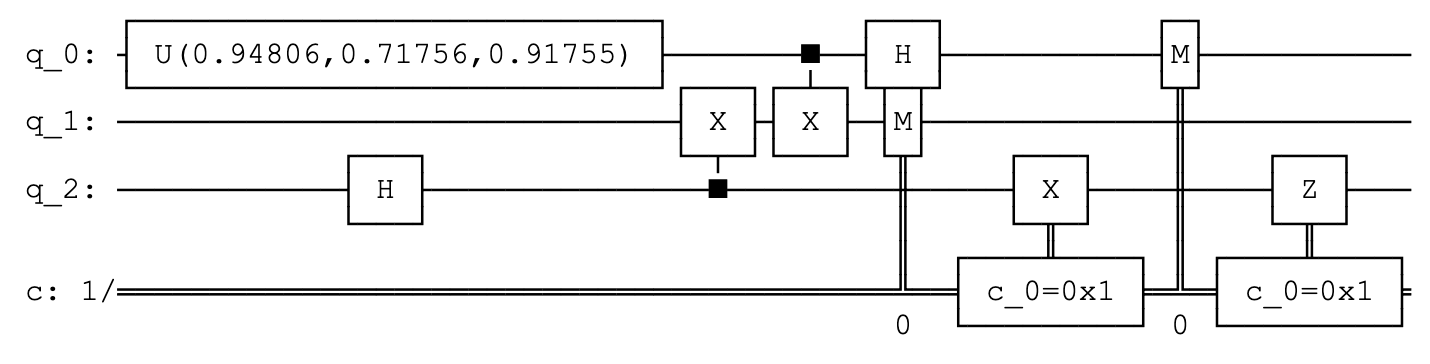
\includegraphics[width=0.9\textwidth]{qtele.png}
    \caption{\label{fig:qtele}2(a) Quantum Teleportation Circuit.}
    \end{figure}
   
   \item Validation Solution 1 : Simulating Statevector
   
   Next, I used statevector-simulator to check the result. I plotted the bloch sphere and used np.vdot to check verify twice. The bloch sphere are both as below.
    \begin{figure}[h]
    \centering
    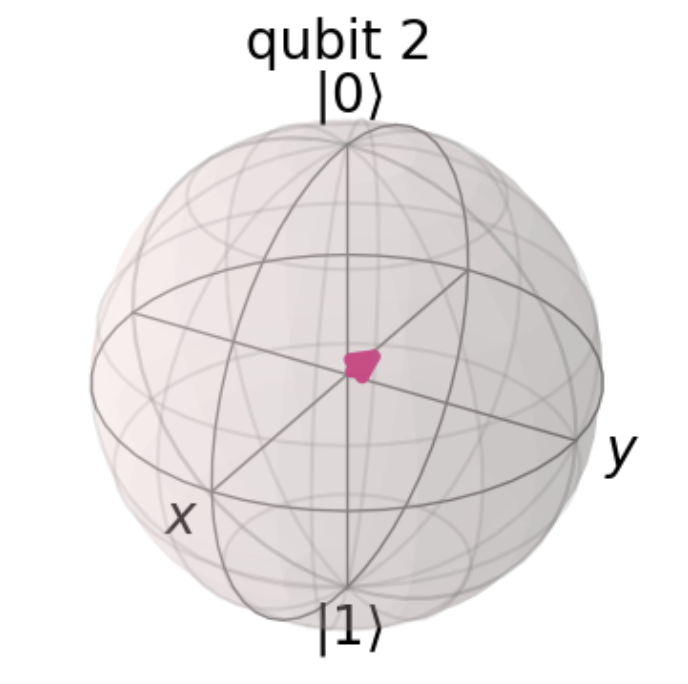
\includegraphics[width=0.4\textwidth]{2asol1.png}
    \caption{\label{fig:2asol1}2(a) bloch sphere figure.}
    \end{figure}
   
    Also, the statevector are both  $Statevector =\begin{bmatrix}
    0.889 & 0.34+0.3j 
    \end{bmatrix} $
    After inner product, we get
    
    $\lvert \prec \phi_B \mid \phi_B \succ \rvert^2 = 1$

    \item Validation Solution 2 : Inverse operation 
    
    In this case, the inverse operation of the qubit state $U^{-1}$ is simply rotating the negative angles of the parameters $(\phi, \theta, \lambda)$
    After simulating, I got the result {'1':6,'0':1018}.
    
    \item Validation Solution 3 : Swap test
    
    In order to implement swap test after teleportation, I combined the two circuits together. With qubit 0 as the perfect teleportation through I-gate, qubit 1-3 for teleportation and qubit 0,3,4 to perform swap test to check the similarity of qubit 0 and 3.The circuit is as below.
    \begin{figure}[h]
    \centering
    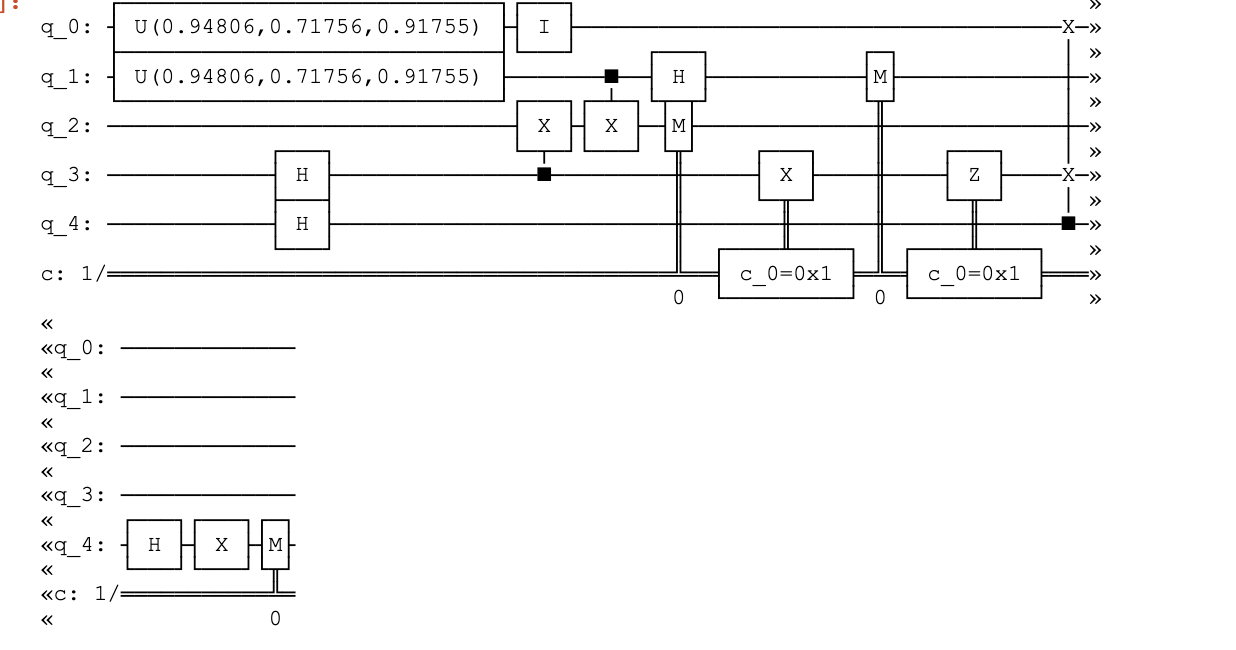
\includegraphics[width=0.9\textwidth]{2asol3.png}
    \caption{\label{fig:2asol3}2(a) Swap Test After Quantum Teleportation Circuit.}
    \end{figure}
    
    The implementing code are in \emph {Appendix 4}
    
    The measured output is {'1':1024}, which supports that the two qubit states are identical.
    
\end{enumerate}

\subsection{(b)}
 I implemented the entanglement swapping protocol as below
    \begin{figure}[h]
    \centering
    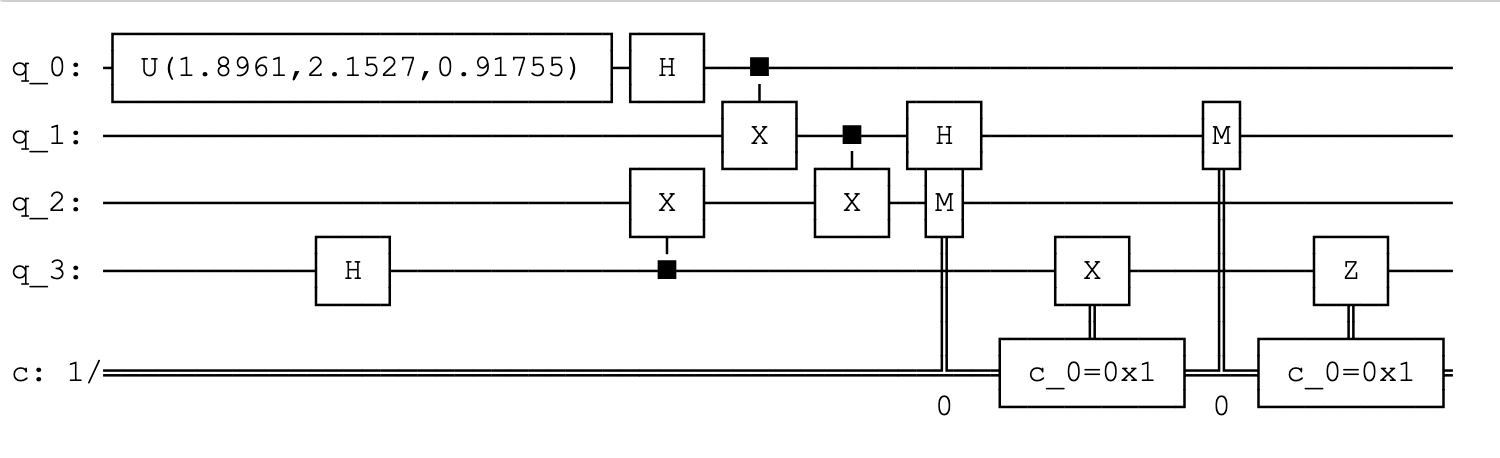
\includegraphics[width=0.9\textwidth]{2bcir.png}
    \caption{\label{fig:2bcir}2(b) Entanglement Swapping Protocol.}
    \end{figure}

After transmitting, the resulting states are as the bloch spheres below. We can see that the 0,3 qubits are in the same state.
    \begin{figure}[h]
    \centering
    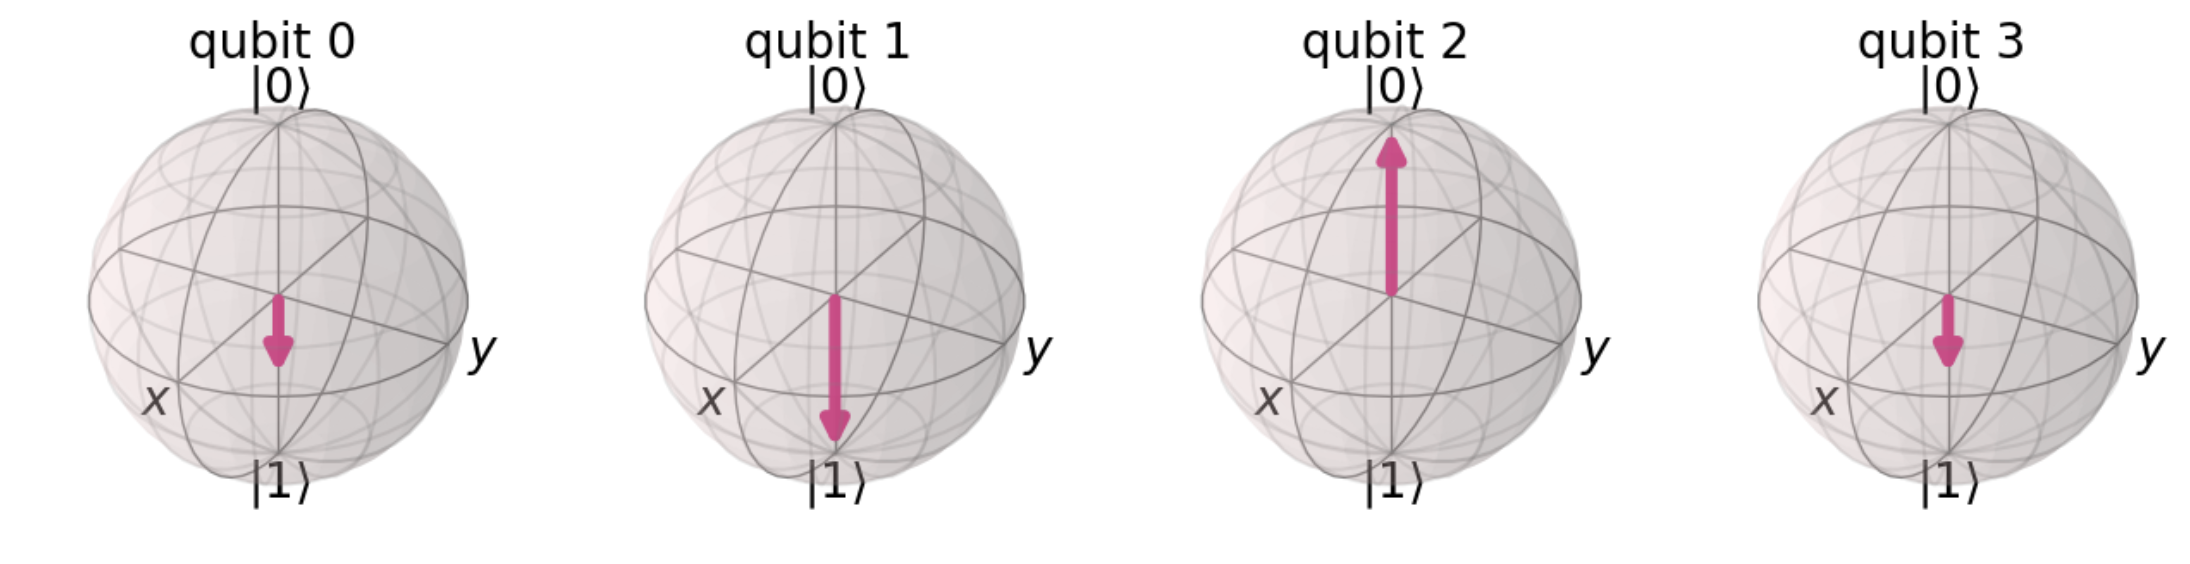
\includegraphics[width=0.9\textwidth]{2bfig.png}
    \caption{\label{fig:2bfig}3(a) Entanglement Swapping Protocol Result.}
    \end{figure}

The implementing code are in \emph {Appendix 5}
\section{The BB84 Protocol}
\subsection{(a)}
The BB84 protocol are implemented as in the source code ipynb(not listed in appendix to prevent redundancy), which I refer to the lab instruction and the Qiskit textbook.

Some points that I found out when understanding the procedure are:
\begin{enumerate}
    \item Just as the instruction guides, I use the same function as intercept-message and measure-message. Because they both are trying to guess the original message
    \item The remove-garbage function does only comparing the basis of encoding and decoding a specific bit. If it is identical, the message decoded is correct and return out.
    \item As to this question, I implemented a simple function to calculate the correct-rate just by brute-force comparing. The result is $ c \approx 0.75$.
    As explained in the Qiskit textbook, the ratio of basis correct-guessing is 0.5, and another 0.25 comes from coincidentally using the wrong basis but came out the correct state.
    \item The reason that Alice and Bob will discard half of the messages in average is simple. It's because the probability to guess the basis correctly is 0.5.

\end{enumerate}

\subsection{(b)}
In order to  measure in Breidbart basis, I implemented a Breidbart-measure function. Using the notion of unitary operation guided in the instruction, I take the approach of Rotation-Y gate. By matrix calculation, the parameter needed(rotation angle $\theta$) is $\frac{\pi}{4}$. The code implementation is in \emph {Appendix 6}. 
The result of the interception is $correct rate \approx 0.75 $.
The reason to this result is as the lab instruction given. The Breidbart basis is the midway basis of computational and x-basis, which gives the 0.5 probability to choose the right basis.
\section{Appendix}
\subsection{Superdense Coding}
\begin{lstlisting}[language=Python]
channel_1 = QuantumCircuit(2,1)
channel_1.h(1)
channel_1.cnot(1,0)
b2 = alice_bits[-2]
b1 = alice_bits[-1]
if(b2 == 1):
    channel_1.z(0)
if(b1 == 1):
    channel_1.x(0)
channel_1.i(0)
channel_1.cnot(0,1)
channel_1.h(0)
channel_1.i(1)
channel_1.measure(0,0) #or channel_1.measure(1,0)
\end{lstlisting}
\subsection{IBM-Q Real Device Superdense Coding Result Histogram}
\begin{figure}[h]
\centering
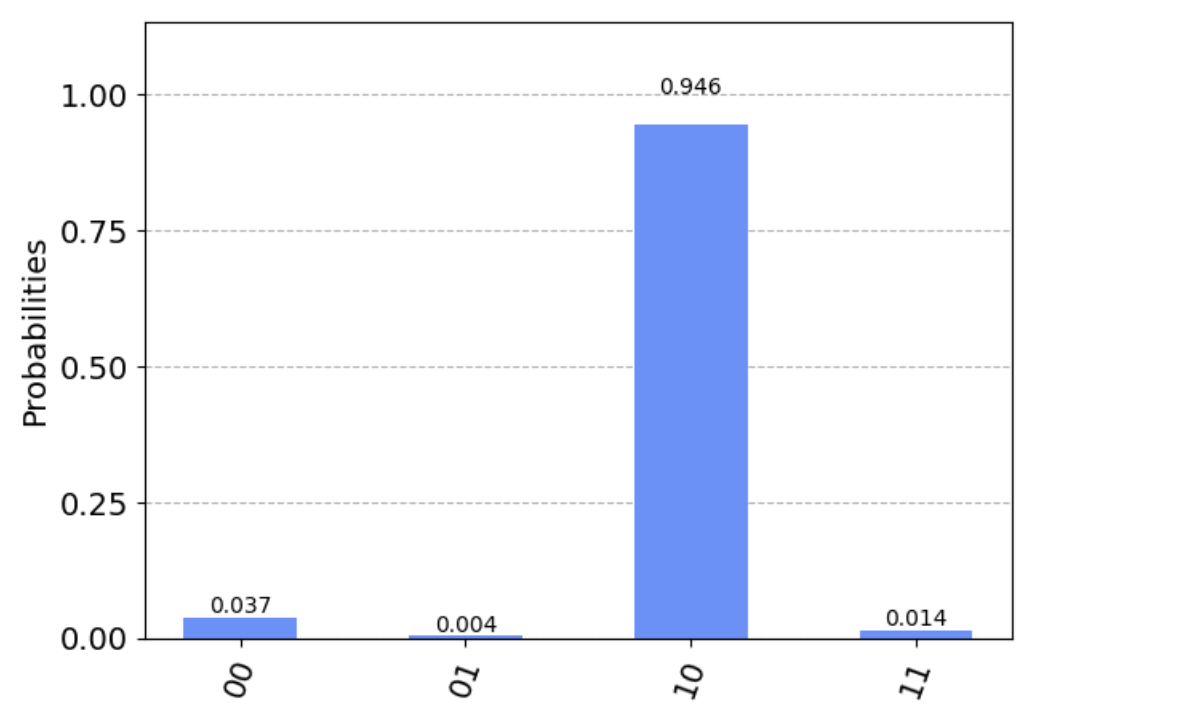
\includegraphics[width=0.7\textwidth]{1b.png}
\caption{\label{fig:1b}1(b) IBM-Q Real Device Superdense Coding Result Histogram.}
\end{figure}
\subsection{Quantum Teleportation}
 \begin{lstlisting}[language = Python]
    qc = QuantumCircuit(3,1)
    qc.u(phi,theta,lamda,0)
    qc.h(2)
    qc.cnot(2,1)
    qc.cnot(0,1)
    qc.h(0)
    qc.measure(1,0)
    qc.x(2).c_if(0, 1)
    qc.measure(0,0)
    qc.z(2).c_if(0, 1)
\end{lstlisting}
\subsection{Swap Test After Quantum Teleportation}
 \begin{lstlisting}[language = Python]
    qc = QuantumCircuit(5,1)
    qc.u(phi,theta,lamda,0)
    qc.i(0)
    qc.u(phi,theta,lamda,1)
    qc.h(3)
    qc.cnot(3,2)
    qc.cnot(1,2)
    qc.h(1)
    qc.measure(2,0)
    qc.x(3).c_if(0, 1)
    qc.measure(1,0)
    qc.z(3).c_if(0, 1)
    #qc.draw()
    
    qc.h(4)
    qc.cswap(4,3,0)
    qc.h(4)
    qc.x(4)
    qc.measure(4,0)
    qc.draw()
\end{lstlisting}
\subsection{Entanglement Swapping Protocol}
 \begin{lstlisting}[language = Python]
    qc2b = QuantumCircuit(4,1)
    qc2b.u(2*phi,3*theta,lamda,0)
    qc2b.h(0)
    qc2b.cnot(0,1)
    qc2b.h(3)
    qc2b.cnot(3,2)
    qc2b.cnot(1,2)
    qc2b.h(1)
    qc2b.measure(2,0)
    qc2b.x(3).c_if(0, 1)
    qc2b.measure(1,0)
    qc2b.z(3).c_if(0, 1)
\end{lstlisting}
\subsection{Breidbart Measurement}
 \begin{lstlisting}[language = Python]
    def Breidbart_measure(message):
        backend = Aer.get_backend('qasm_simulator')
        measurements = []
        for q in range(n):
            message[q].ry(-math.pi/4,0)
            message[q].measure(0,0)
            message[q].ry(math.pi/4,0) # preparing the post-measurement state
            result = execute(message[q], backend, shots=1, memory=True).result() 
            measured_bit = int(result.get_memory()[0]) 
            measurements.append(measured_bit)
        return measurements
\end{lstlisting}

\end{CJK*}
\end{document}
